\documentclass[paper=a4, 12pt, twoside]{article} 
%\usepackage[margin=1in]{geometry}          
\usepackage{graphicx}
\usepackage{apacite}
\setlength\bibitemsep{1.5\itemsep} %sets spacing between reference entries

\usepackage{caption}
\captionsetup{font=bf}

\usepackage{amsthm, amsmath, amssymb}
\usepackage{setspace}\doublespacing
\usepackage[loose,nice]{units} %replace "nice" by "ugly" for units in upright fractions
\usepackage{booktabs}
\usepackage[table,xcdraw]{xcolor}
\usepackage[top=2.54cm, bottom=2.54cm, left=2.54cm, right=2.54cm]{geometry} %margin control
\linespread{1.0} % 1.3 for one-and-half spacing
\parskip  3mm
\usepackage{fancyhdr} % create header
\setlength{\headheight}{10pt}
\pagestyle{fancy}
\fancyhf{} % removes previous header
% Even Page Header
\fancyhead[EL]{\footnotesize \thepage}
%\fancyhead[EC]{\footnotesize Mohammed Quazi, Yan Lu}
%\fancyhead[ER]{\footnotesize [Vol. 18, No. 1} %{[Spl. Vol.}
% Odd Page Header
%\fancyhead[OL]{\footnotesize 2020]}
%\fancyhead[OC]{\footnotesize Adjusted Design Effect Model for Individual Variables in Survey Data}
\fancyhead[OR]{\footnotesize \thepage}
\renewcommand{\headrulewidth}{0pt} % 0pt thickness eliminates headrule

% front Page Footer (no header in front page)
\fancypagestyle{frontpagefooter}{%
	\fancyhead{} % eliminates all header used elsewhere
	\renewcommand{\footrulewidth}{0.4pt}   % a thin line to separate main text and footer
	\fancyfoot[L]{\footnotesize 
		\footnote{a}Department of Mathematics and Statistics, University of New Mexico
	}
	\fancyfoot[C]{\footnotesize }	  
	%\fancyfoot[R]{\footnotesize \thepage} 	
}
\setcounter{page}{1} % The Editorial Office will change this value as needed
%\setlength{\oddsidemargin}{0in}
%\setlength{\evensidemargin}{0in}
%\setlength{\topmargin}{-.5in}
%\setlength{\headsep}{0in}
%\setlength{\textwidth}{6.5in}
%\setlength{\textheight}{8.5in}
%\def\refhg{\hangindent=20pt\hangafter=1}
%\def\refmark{\par\vskip 2mm\noindent\refhg}
%\def\refhg{\hangindent=20pt\hangafter=1}
%\def\refmark{\par\vskip 2mm\noindent\refhg}
%\def\refhg{\hangindent=20pt\hangafter=1}    %20pt
%\def\refhgb{\hangindent=10pt\hangafter=1}
%\def\refmark{\par\vskip 2mm\noindent\refhg}
%\renewcommand{\baselinestretch}{1.5}
\usepackage[symbol*]{footmisc}
\DefineFNsymbolsTM{myfnsymbols}{% def. from footmisc.sty "bringhurst" symbols
	\textasteriskcentered *
	\textdagger    \dagger
	\textdaggerdbl \ddagger
	\textsection   \mathsection
	\textbardbl    \|%
	\textparagraph \mathparagraph
}%
\setfnsymbol{myfnsymbols}
\usepackage{sectsty}
\usepackage{indentfirst}
\sectionfont{\fontsize{12}{15}\selectfont}

\begin{document}
	\thispagestyle{empty}
	\thispagestyle{frontpagefooter}
	
%	% For a regular issue 
%	\noindent{Statistics and Applications {\bf \{ISSN 2452-7395(online)\} } \\
%		Volume 18, No. 1 (New Series), pp. 1--21} % Editorial Office will change VOLUME, ISSUE and PAGE numbers
	
	% For a Special Volume % Comment out above 2 lines, and uncomment below 2 lines
	% \noindent {\it %Special Proceeding of the 22\,$^{nd}$ Annual Conference of SSCA held at Savitribai Phule\\ 
	% Pune University, Ganeshkhind, Pune, MH, during January 02--04, 2020; pp 1--20}
	% %Editorial Office will change VOLUME, ISSUE and PAGE numbers
	\begin{center} 
		{\fontsize{18}{24} \selectfont % DO NOT CHANGE FONTSIZE
			{\bf Survey Sampling and Cricket: Predicting the\\[2mm] `Gentleman's Game'}} \\[6mm]
%		[2mm] % YOU CAN USE MULTIPLE LINES
%				in Survey Data} } \\[6mm] % BIGGER GAP NEEDED HERE, DO NOT CHANGE
		\normalsize
		{\bf Mohammed Quazi$^{*}$, Pavan Datta$^{*}$, Joshua Clifford$^{*}$} \\
%		{\it Department of Mathematics and Statistics \\
%			University of New Mexico, Albuquerque, New Mexico, USA} \\[6mm] % BIGGER GAP NEEDED, DO NOT CHANGE
		
%		Received: 26 March 2020; Revised: 15 April 2020; Accepted: 20 April 2020 % Editorial Office will determine dates
	\end{center}
	%  	\renewcommand{\footnoterule}{%
	% 	\kern 2pt
	% 	\hrule width \textwidth height 0.4pt
	% 	\kern 2pt
	% }
	\vspace{-8mm}
	
	\noindent\rule{16.5cm}{0.8pt}
	\vspace{-5mm}
%	\begin{abstract}
%		dgdgfd
%	\end{abstract}
\section*{\centerline{Abstract}}
%	\noindent{\textbf{Abstract}}\vspace{-1mm}
	
	\setlength\parindent{0pt}
	
	% 	\title{Adjusted Design Effect Model for Individual Variables in Survey Data}
	%	 \footnote{Mohammed Quazi, Graduate Student ({\textit{mquazi@unm.edu}})}, \footnote{Yan Lu, Associate Professor ({\textit{yanlu@unm.edu}})} 
	%% 	\renewcommand\footnoterule{\rule{16.5cm}{0.4pt}}
	% \date{}
	%\begin{abstract}\label{abstract}
%\begin{abstract}\label{abstract}
	\section*{Introduction}\label{intro}
		The 2019 Men’s International Cricket Council (ICC) Cricket World Cup (CWC) was the most watched ICC event of all time, with a 1.6 billion cumulative average audience for
		live coverage, a 38\% increase over the 2015 edition. This research develops a statistical
		modeling procedure to predict outcomes of future ICC cricket events. The proposed
		model provides an insight into the application of survey sampling to the team selection
		pattern by incorporating individual players' performance history not only against a
		particular opposition but also against any cricket-playing nation (full member of ICC).
		A case study for the next ICC CWC 2023 in India is provided, and simulation results are
		discussed.  
	\section*{Methods}\label{method}
		This study employs stratified random sampling  (SRS) technique shown in Figure \ref{samplingscheme} to select team lineups based on player roles. \textit{S1-S6} denote different types of players based on their role in the team - fast bowler, spinner, all-rounder-fast bowler, all-rounder-spinner, batsman, wicket-keeper. Runs scored by each player on the team is derived using an algorithm based off of estimating parameters of a gamma distribution against a particular opposition, which is then used to simulate match and tournament results. Web scraped data collected spans over 11000 individual one-day international (ODI) innings that cover every competitive game played among the full members of ICC since 1999. 195 international players are considered for the case study. The proposed model accounts for the Indian subcontinent playing conditions and debutants' performances. 
			\section*{Results}\label{results}
		Figure \ref{joshplot} shows the probability distribution for standings based on points accumulated at the end of group stage of ICC CWC 2023, after which the top 4 teams qualify for the semifinals. Table \ref{table22} shows the predicted probability of winning for teams against each other. Results indicate that India has the highest chance of qualifying for the semis and a 24\% chance of winning the cup. Nevertheless, surprisingly, Pakistan are the favorites, with a 52\% chance of winning the trophy if they make it to the semifinals, living up to their `unpredictable' tag and setting up a replay of the ICC Champions Trophy Final in 2017, which they won despite being underdogs against India. South Africa (another  heavy favorite with) are likely to shed their reputation for choking and qualify for the semis, with a 9\% chance of winning the tournament.   
			\section*{Conclusion}\label{conclusion}
		 The method can predict probabilities of winning, which is of interest to fans and also could inform setting gambling odds. The method can also be adapted to recommend team selection strategies to inform teams' approaches to increase chances of success in a game. This study could be applied to all league-format cricket tournaments, including the Indian Premier League (IPL) -- one of the top 10 most watched sports leagues in the world (average attendance) and the most attended and watched cricket league in the world. The proposed model could be implemented for other sports as well. \\
		 (Word count 483/500)
%	\wordcount 
%\end{abstract}
\cleardoublepage
 \begin{figure}[h]
	\centering
	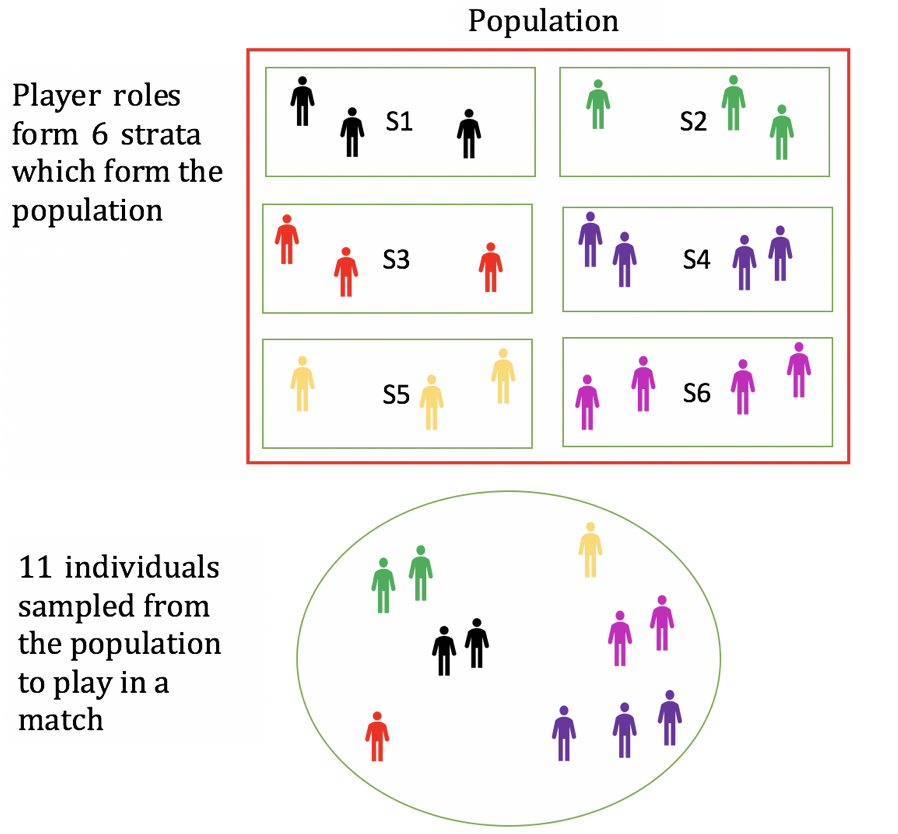
\includegraphics[scale=0.70]{samplingscheme} 
	\caption{Sampling scheme employed in this study. S1-S6 are strata. Oval shows individuals sampled using stratified random sampling method. }
	\label{samplingscheme}
\end{figure}
 \begin{figure}[h]
	\centering
	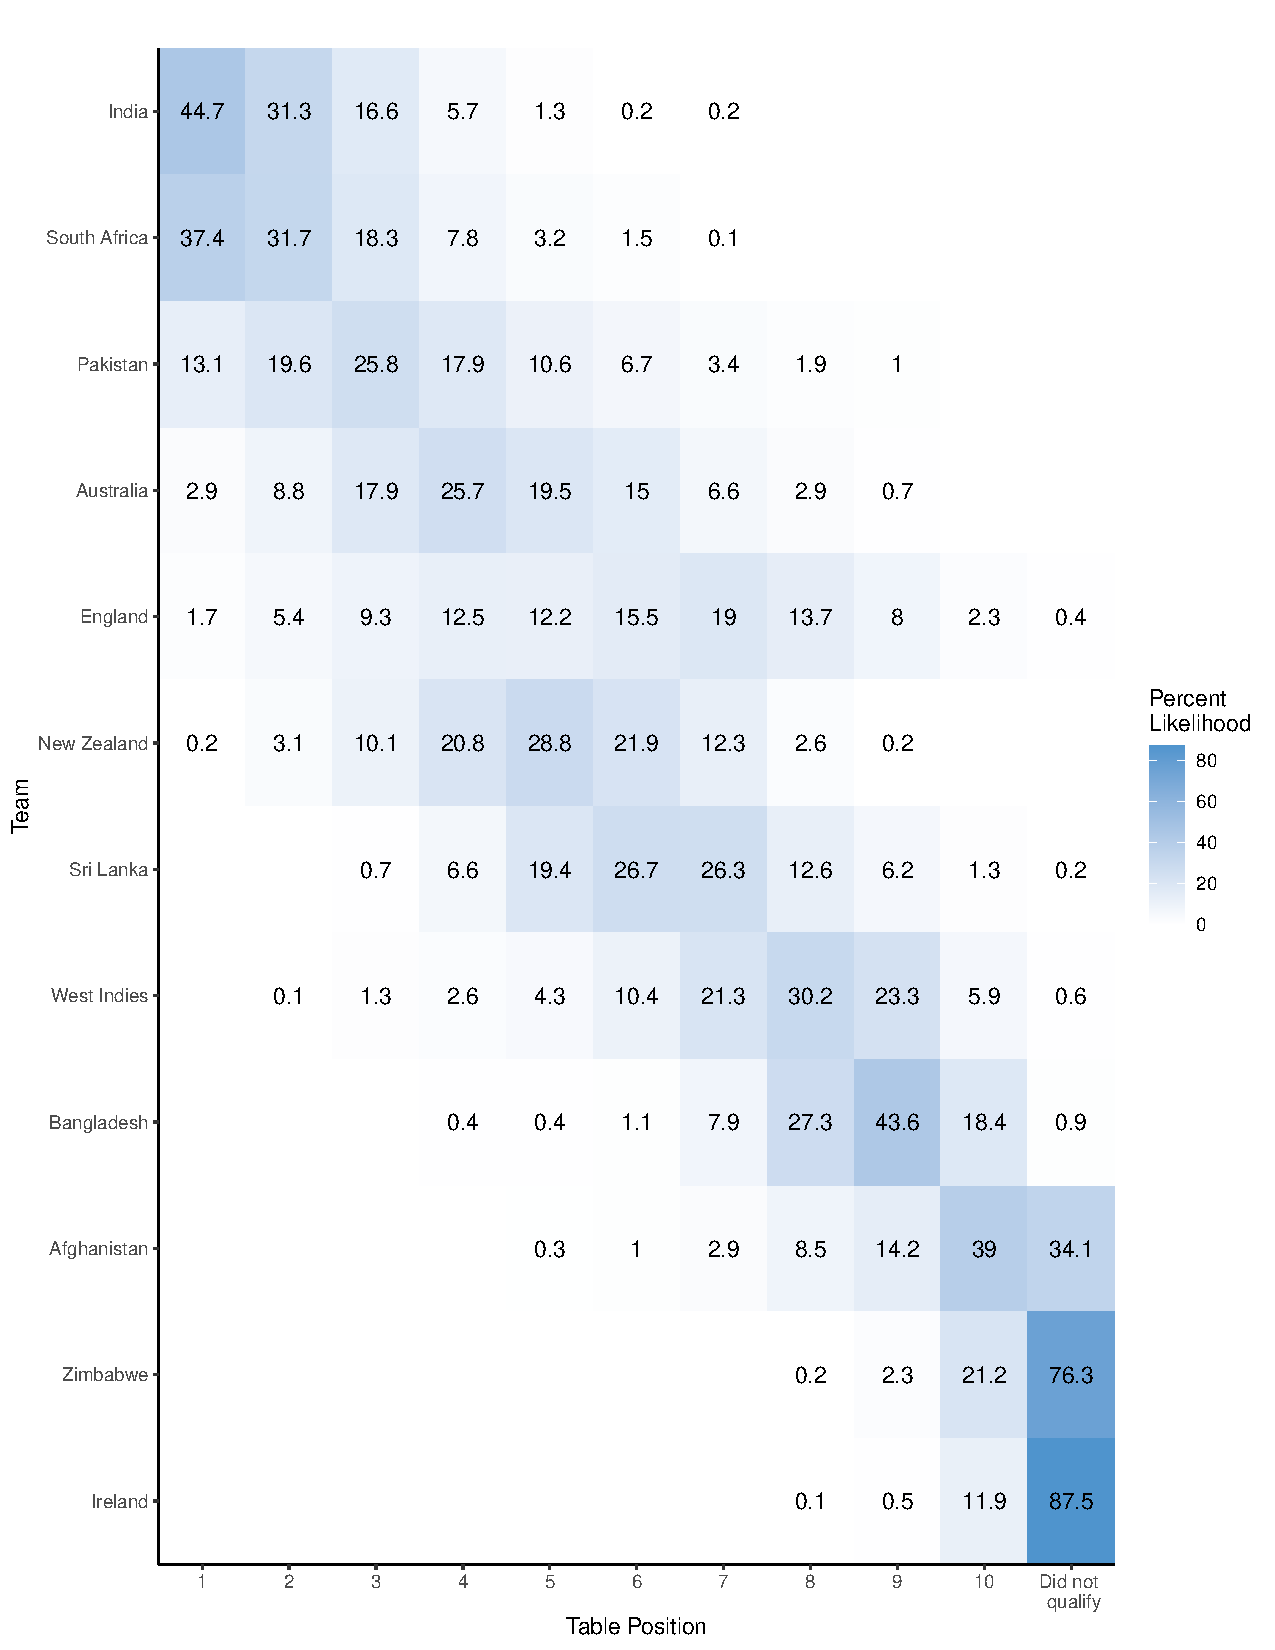
\includegraphics[scale=0.60]{cricket_plot.pdf} 
	\caption{ICC 2023 World Cup Team Table Probability Distribution}
	\label{joshplot}
\end{figure}
% Please add the following required packages to your document preamble:
% \usepackage{booktabs}
% \usepackage{graphicx}
%table 1 begins here
%\begin{table}[]
%	\centering
%	\caption{Probability distribution (in \%) for team standings at the ICC 2023 CWC - Ireland and Zimbabwe are least likely to qualify for the world cup}
%	\label{table1}
%	\resizebox{\textwidth}{!}{%
%		\begin{tabular}{@{}lccccccccccccc@{}}
%			\toprule
%			\multicolumn{14}{c}{\textbf{Team Standings}}                                                         \\
%			\textbf{Teams} &
%			\textbf{1} &
%			\textbf{2} &
%			\textbf{3} &
%			\textbf{4} &
%			\textbf{5} &
%			\textbf{6} &
%			\textbf{7} &
%			\textbf{8} &
%			\textbf{9} &
%			\textbf{10} &
%			\textbf{11} &
%			\textbf{12} &
%			\textbf{\begin{tabular}[c]{@{}c@{}}Aggregate \\
%					 Standings\end{tabular}} \\
%				 			\toprule
%			Afghanistan  & 0    & 0    & 0    & 0    & 0.3  & 1    & 2.9  & 8.5  & 14.2 & 39   & 25.7 & 8.4  & 10 \\
%			Australia    & 2.9  & 8.8  & 17.9 & 25.7 & 19.5 & 15   & 6.6  & 2.9  & 0.7  & 0    & 0    & 0    & 4  \\
%			Bangladesh   & 0    & 0    & 0    & 0.4  & 0.4  & 1.1  & 7.9  & 27.3 & 43.6 & 18.4 & 0.9  & 0    & 9  \\
%			England      & 1.7  & 5.4  & 9.3  & 12.5 & 12.2 & 15.5 & 19   & 13.7 & 8    & 2.3  & 0.4  & 0    & 5  \\
%			India        & 44.7 & 31.3 & 16.6 & 5.7  & 1.3  & 0.2  & 0.2  & 0    & 0    & 0    & 0    & 0    & 1  \\
%			Ireland      & 0    & 0    & 0    & 0    & 0    & 0    & 0    & 0.1  & 0.5  & 11.9 & 27.7 & 59.8 & 12 \\
%			New Zealand  & 0.2  & 3.1  & 10.1 & 20.8 & 28.8 & 21.9 & 12.3 & 2.6  & 0.2  & 0    & 0    & 0    & 6  \\
%			Pakistan     & 13.1 & 19.6 & 25.8 & 17.9 & 10.6 & 6.7  & 3.4  & 1.9  & 1    & 0    & 0    & 0    & 3  \\
%			South Africa & 37.4 & 31.7 & 18.3 & 7.8  & 3.2  & 1.5  & 0.1  & 0    & 0    & 0    & 0    & 0    & 2  \\
%			Sri Lanka    & 0    & 0    & 0.7  & 6.6  & 19.4 & 26.7 & 26.3 & 12.6 & 6.2  & 1.3  & 0.2  & 0    & 7  \\
%			West Indies  & 0    & 0.1  & 1.3  & 2.6  & 4.3  & 10.4 & 21.3 & 30.2 & 23.3 & 5.9  & 0.6  & 0    & 8  \\
%			Zimbabwe     & 0    & 0    & 0    & 0    & 0    & 0    & 0    & 0.2  & 2.3  & 21.2 & 44.5 & 31.8 & 11 \\ \bottomrule
%		\end{tabular}%
%	}
%\end{table}
%table 1 ends here
% Please add the following required packages to your document preamble:
% \usepackage{booktabs}
% \usepackage{graphicx}
\begin{table}[]
		\centering
	\caption{Predicted win/loss ratio (in \%) at the ICC 2023 CWC}
	\label{table22}
	\resizebox{\textwidth}{!}{%
		\begin{tabular}{@{}lllllllllllll@{}}
			\toprule
			\multicolumn{13}{c}{\textbf{Losing team}}                                                                             \\
			\multicolumn{1}{l|}{\textbf{Winning team}} &
			Afghanistan &
			Australia &
			Bangladesh &
			England &
			India &
			Ireland &
			New Zealand &
			Pakistan &
			South Africa &
			Sri Lanka &
			West Indies &
			Zimbabwe \\ \cmidrule(l){2-13} 
			\multicolumn{1}{l|}{Afghanistan}  &      & 0.20 & 41.1 & 4.20 & 0.00 & 95.7 & 0.70 & 30.1 & 0.00 & 8.70 & 20.3 & 47.9 \\
			\multicolumn{1}{l|}{Australia}    & 99.8 &      & 86.2 & 61.0 & 63.8 & 100  & 99.5 & 25.6 & 0.90 & 7.30 & 86.3 & 100  \\
			\multicolumn{1}{l|}{Bangladesh}   & 58.5 & 13.6 &      & 2.10 & 2.60 & 100  & 0.80 & 13.4 & 0.20 & 2.30 & 94.9 & 100  \\
			\multicolumn{1}{l|}{England}      & 95.8 & 37.7 & 97.9 &      & 10.8 & 93.8 & 66.7 & 37.2 & 12.5 & 33.1 & 37.1 & 90.2 \\
			\multicolumn{1}{l|}{India}        & 100  & 35.6 & 97.4 & 88.9 &      & 100  & 100  & 67.7 & 39.4 & 99.9 & 99.3 & 100  \\
			\multicolumn{1}{l|}{Ireland}      & 3.90 & 0.00 & 0.00 & 5.80 & 0.00 &      & 0.00 & 0.00 & 0.00 & 32.2 & 0.00 & 39.5 \\
			\multicolumn{1}{l|}{New Zealand}  & 99.3 & 0.50 & 99.0 & 32.2 & 0.00 & 100  &      & 85.3 & 19.0 & 100  & 56.8 & 89.3 \\
			\multicolumn{1}{l|}{Pakistan}     & 68.8 & 73.0 & 86.4 & 61.9 & 31.7 & 100  & 14.3 &      & 88.7 & 100  & 79.4 & 100  \\
			\multicolumn{1}{l|}{South Africa} & 100  & 99.0 & 99.8 & 87.2 & 59.4 & 100  & 80.4 & 11.0 &      & 100  & 72.8 & 100  \\
			\multicolumn{1}{l|}{Sri Lanka}    & 90.1 & 92.6 & 97.5 & 66.3 & 0.10 & 67.2 & 0.00 & 0.00 & 0.00 &      & 71.1 & 99.6 \\
			\multicolumn{1}{l|}{West Indies}  & 79.2 & 13.3 & 4.80 & 61.9 & 0.70 & 100  & 42.4 & 19.9 & 26.8 & 27.5 &      & 97.1 \\
			\multicolumn{1}{l|}{Zimbabwe}     & 49.9 & 0.00 & 0.00 & 9.50 & 0.00 & 59.6 & 9.80 & 0.00 & 0.00 & 0.40 & 2.80 &  \\ \bottomrule   
		\end{tabular}%
	}
\end{table}
% Please add the following required packages to your document preamble:
% \usepackage{booktabs}
% \usepackage{graphicx}
\begin{table}[]
	\centering
	\caption{All time win/loss ratio (in \%)}
	\label{table33}
	\resizebox{\textwidth}{!}{%
		\begin{tabular}{@{}lllllllllllll@{}}
			\toprule
\multicolumn{13}{c}{\textbf{Losing team}}                                                                             \\
			\multicolumn{1}{l|}{\textbf{Winning team}} &
			Afghanistan &
			Australia &
			Bangladesh &
			England &
			India &
			Ireland &
			New Zealand &
			Pakistan &
			South Africa &
			Sri Lanka &
			West Indies &
			Zimbabwe \\ \cmidrule(l){2-13} 
			\multicolumn{1}{l|}{Afghanistan}  &      & 0.00 & 37.5 & 0.00 & 16.7 & 50.0 & 0.00 & 0.00 & 0.00 & 25.0 & 37.5 & 60.0 \\
			\multicolumn{1}{l|}{Australia}    & 100  &      & 95.0 & 56.8 & 60.0 & 100  & 70.2 & 67.8 & 48.5 & 65.6 & 55.1 & 93.1 \\
			\multicolumn{1}{l|}{Bangladesh}   & 62.5 & 5.00 &      & 19.0 & 14.3 & 77.8 & 28.6 & 13.5 & 19.0 & 15.2 & 41.7 & 62.7 \\
			\multicolumn{1}{l|}{England}      & 100  & 43.2 & 81.0 &      & 44.3 & 83.3 & 48.9 & 62.4 & 48.3 & 50.0 & 54.2 & 72.4 \\
			\multicolumn{1}{l|}{India}        & 83.3 & 40.0 & 85.7 & 55.7 &      & 100  & 52.9 & 43.0 & 43.2 & 61.8 & 50.4 & 82.5 \\
			\multicolumn{1}{l|}{Ireland}      & 50.0 & 0.00 & 22.2 & 16.7 & 0.0  &      & 0.00 & 21.4 & 0.00 & 0.00 & 9.09 & 50.0 \\
			\multicolumn{1}{l|}{New Zealand}  & 100  & 29.8 & 71.4 & 51.1 & 47.1 & 100  &      & 46.6 & 37.9 & 54.4 & 48.3 & 74.3 \\
			\multicolumn{1}{l|}{Pakistan}     & 100  & 32.2 & 86.5 & 37.6 & 57.0 & 78.6 & 53.4 &      & 35.9 & 61.3 & 45.9 & 92.1 \\
			\multicolumn{1}{l|}{South Africa} & 100  & 51.5 & 81.0 & 51.7 & 56.8 & 100  & 62.1 & 64.1 &      & 58.6 & 74.2 & 95.0 \\
			\multicolumn{1}{l|}{Sri Lanka}    & 75.0 & 34.4 & 84.8 & 50.0 & 38.2 & 100  & 45.6 & 38.7 & 41.4 &      & 50.9 & 80.0 \\
			\multicolumn{1}{l|}{West Indies}  & 62.5 & 44.9 & 58.3 & 45.8 & 49.6 & 90.9 & 51.7 & 54.1 & 25.8 & 49.1 &      & 77.7 \\
			\multicolumn{1}{l|}{Zimbabwe}                         & 40.0 & 6.89 & 37.3 & 27.6 & 17.5 & 50.0 & 25.7 & 7.89 & 5.00 & 20.0 & 22.3 &      \\ \bottomrule
		\end{tabular}%
	}
\end{table}
\end{document}